\chapter[Elements of Image Processing with \texttt{{R}}]{Elements of Image Processing with \texttt{{R}}}\label{Chapter:ElementsR}

\section{Statistics and Image Processing}

A nice example of what can be accomplished with \texttt R is a very useful operation which is a commodity in image processing: histogram equalization.
More often than not, the images we deal with have a huge dynamic range.
Consider, for instance Listing~\ref{Code:SummaryStatistics} (page~\pageref{Code:SummaryStatistics}).
The ranges are 
$(1,526287)$, $(0.004,15723.672) $, and $(0.17,134204.69)$ for the HH, HV and VV bands, respectively.
As seen in Fig.~\ref{Fig:BoxplotDark} (page~\pageref{Fig:BoxplotDark}), the values are fairly concentrated in the lower part.
If we simply map the minima and maxima to black and white, and linearly the intermediate values into gray levels, both individual bands and any composite image will look black.
We wonder if we can improve visualization by better distributing the values, and in order to do so we will rely on a result from probability theory.

\begin{theorem}\label{Theo:FZ}
Consider the continuous random variable $Z\colon \Omega\to\mathbbm R$ with cumulative distribution function $F_Z$.
The random variable $W=F_Z(Z)$ has uniform distribution.
\end{theorem}

\begin{proof}
The cumulative distribution function of $W$ is $F_W(w)=\Pr(W\leq w)=\Pr(F_Z(Z)\leq w)$.
Since $Z$ is continuous, there exists the inverse of its cumulative distribution function, $F^{-1}_Z$.
We can then write 
$F_W(w)=\Pr(F_Z(Z)\leq w) = \Pr(F^{-1}_Z(F_Z(Z)) \leq F^{-1}(w)) = \Pr(Z\leq F^{-1}_Z(w))$, 
which is exactly the cumulative distribution function of $Z$ at $F^{-1}_Z(w)$, so $F_W(w)=F_Z(F^{-1}_Z(w))=w$, which characterizes a uniform random variable on $(0,1)$; cf.\ Eq.~\eqref{eq:CDFUniform}, Section~\ref{Sec:UnifDistribution}.
\end{proof}

So we only need to apply the cumulative distribution function of the random variable that produced the data to the data themselves and we will obtain samples from the Uniform distribution.
But do we have this function?
Usually we don't, but we can estimate it.

One of the simplest manners to estimate a cumulative distribution function from data $\bm z=(z_1,\dots,z_n)$ is with the empirical cumulative distribution function, or just \textit{empirical function}.
It is just the finite approximation of the definition of a cumulative distribution function, and is given by
\begin{equation}
\widehat{F}(t) = \frac1n \#\{j \text{ such that } z_j\leq t\} ,
\end{equation}
where $\#$ denotes the number of elements in the set.

Let's see an example.
Consider the real part of the HH band of Fig.~\ref{Im:Oberpfaffenhofen_RGB}, whose histogram is the top leftmost of Fig.~\ref{Fig:FittedDarkRegion}; assume it is stored in the \verb|HH_Complex| variable.
These data are clearly not uniformly distributed.
We will randomly sample (fixing the pseudorandom number generator and the seed for reproducibility) one hundred observations, and then proceed to build its empirical function.

\begin{lstlisting}[frame=tb]
set.seed(1234567890, kind="Mersenne-Twister")

Z <- sample(as.vector(Re(HH_Complex)), size = 100, replace = FALSE)
W <- ecdf(Z)(Z)

HistogramEqualization <- data.frame(Z,W)
 
ggplot(data=HistogramEqualization, aes(x=Z)) +
  geom_histogram(aes(y = ..density..), col="black", fill="white") +
  xlab("Observations") +
  ylab("Histogram") + 
  theme_few() +
  theme(text = element_text(size=20))

ggplot(data=HistogramEqualization, aes(x=Z)) +
  stat_ecdf(geom="step", pad=FALSE) +
  xlab("Observations") +
  ylab("Empirical Function") + 
  theme_few() +
  theme(text = element_text(size=20))

ggplot(data=HistogramEqualization, aes(x=W)) +
  geom_histogram(aes(y = ..density..), col="black", fill="white") +
  xlab("Equalized Observations") +
  ylab("Histogram") + 
  theme_few() +
  theme(text = element_text(size=20))
\end{lstlisting}

\begin{figure*}[hbt]
\centering
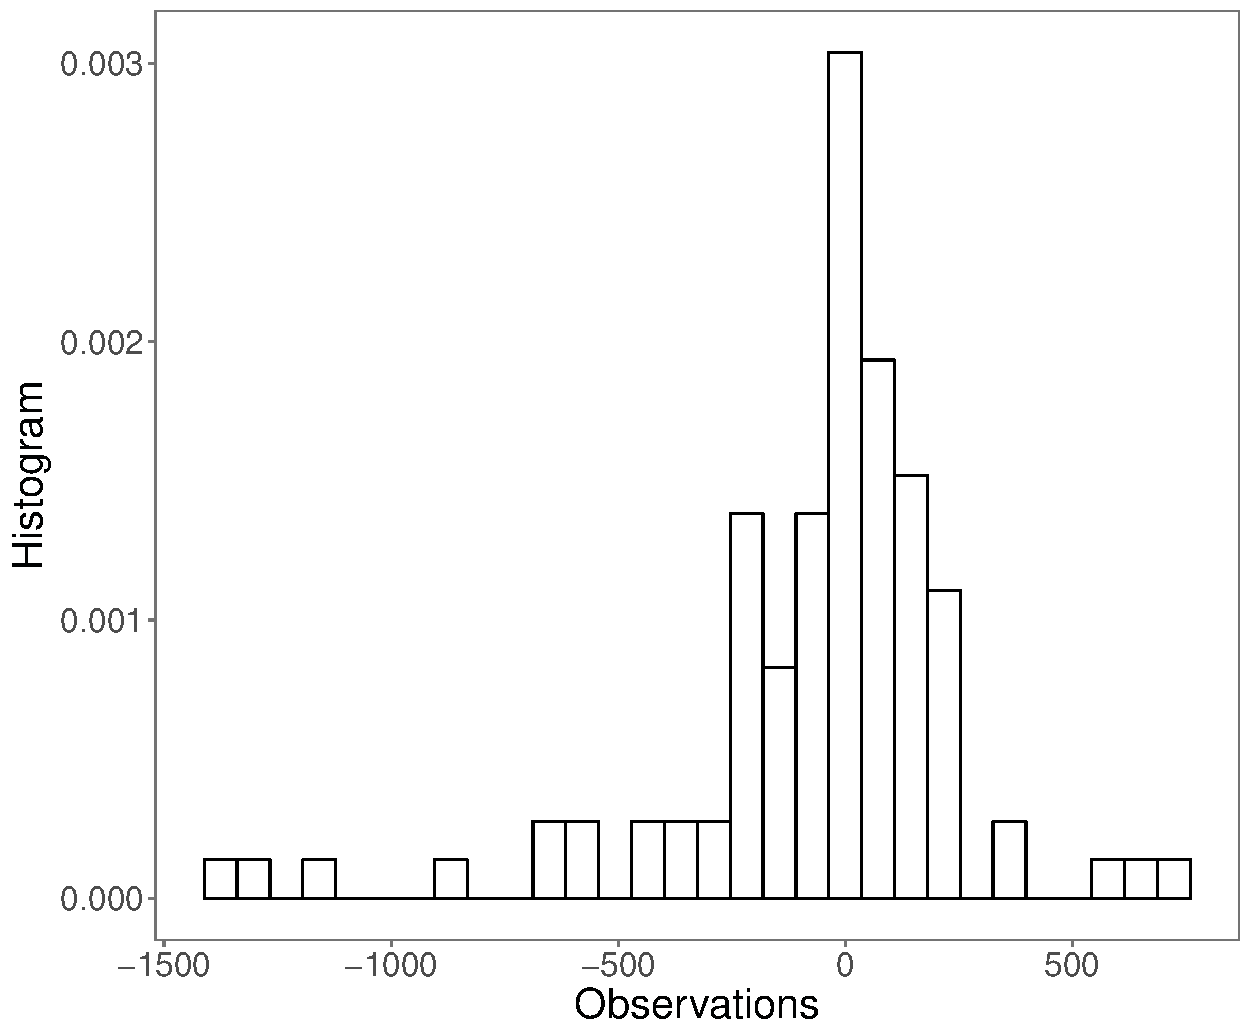
\includegraphics[width=.32\linewidth]{Histogram}
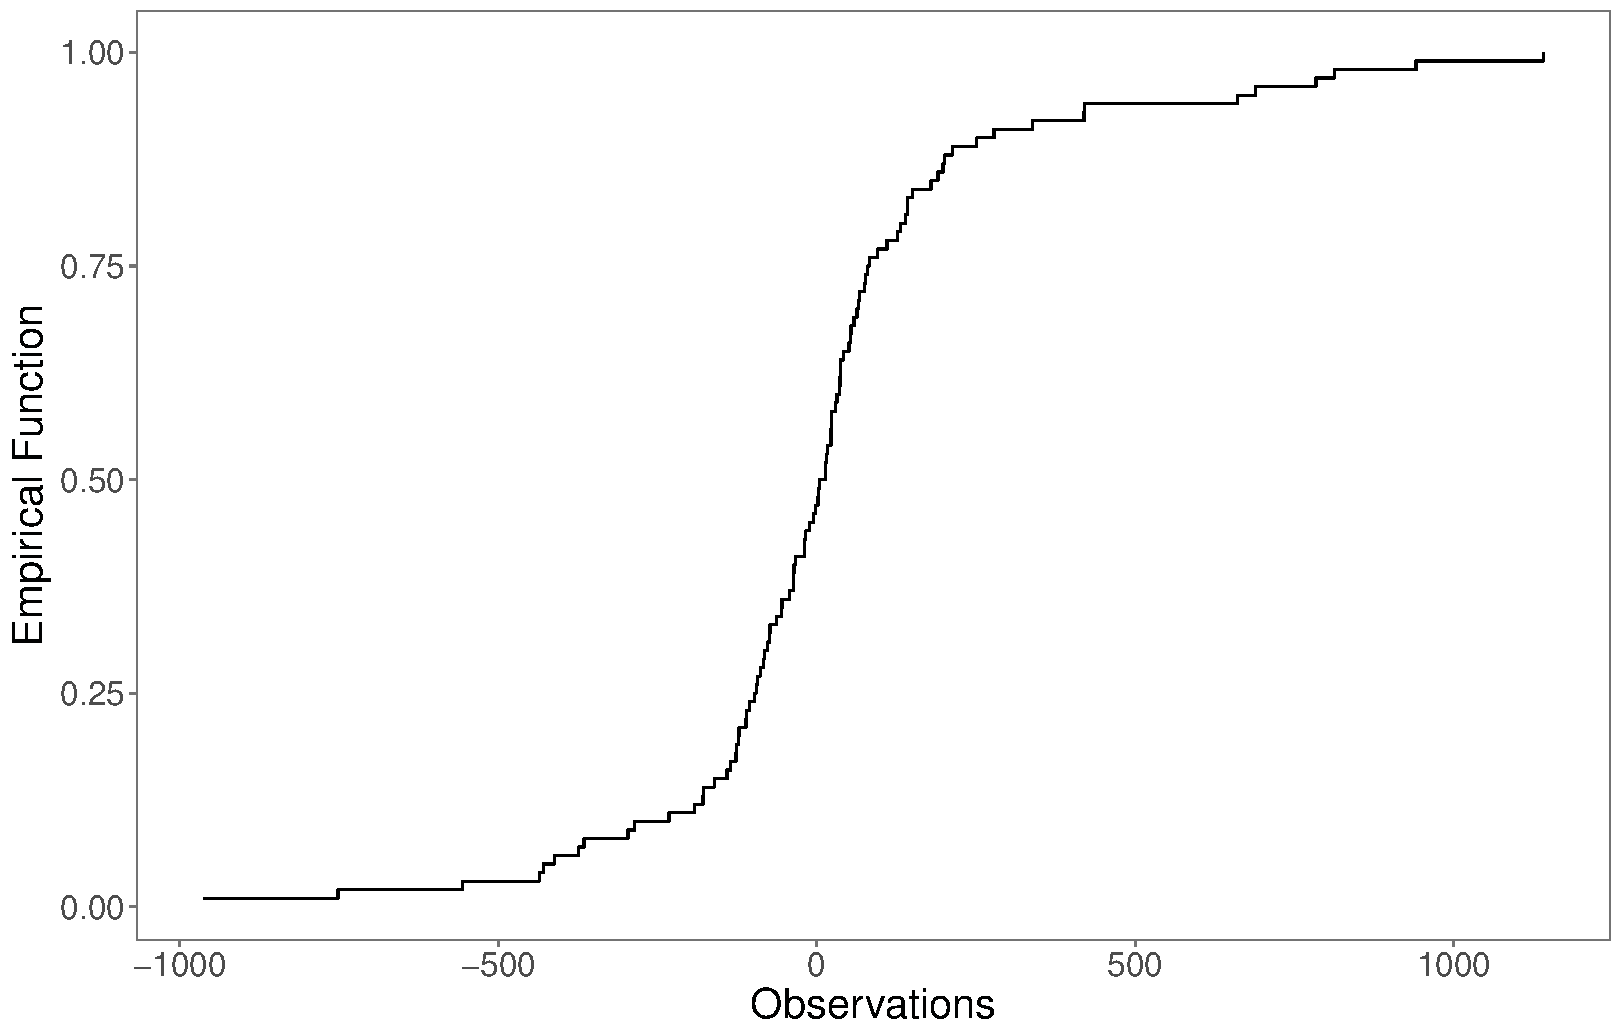
\includegraphics[width=.32\linewidth]{ECDF}
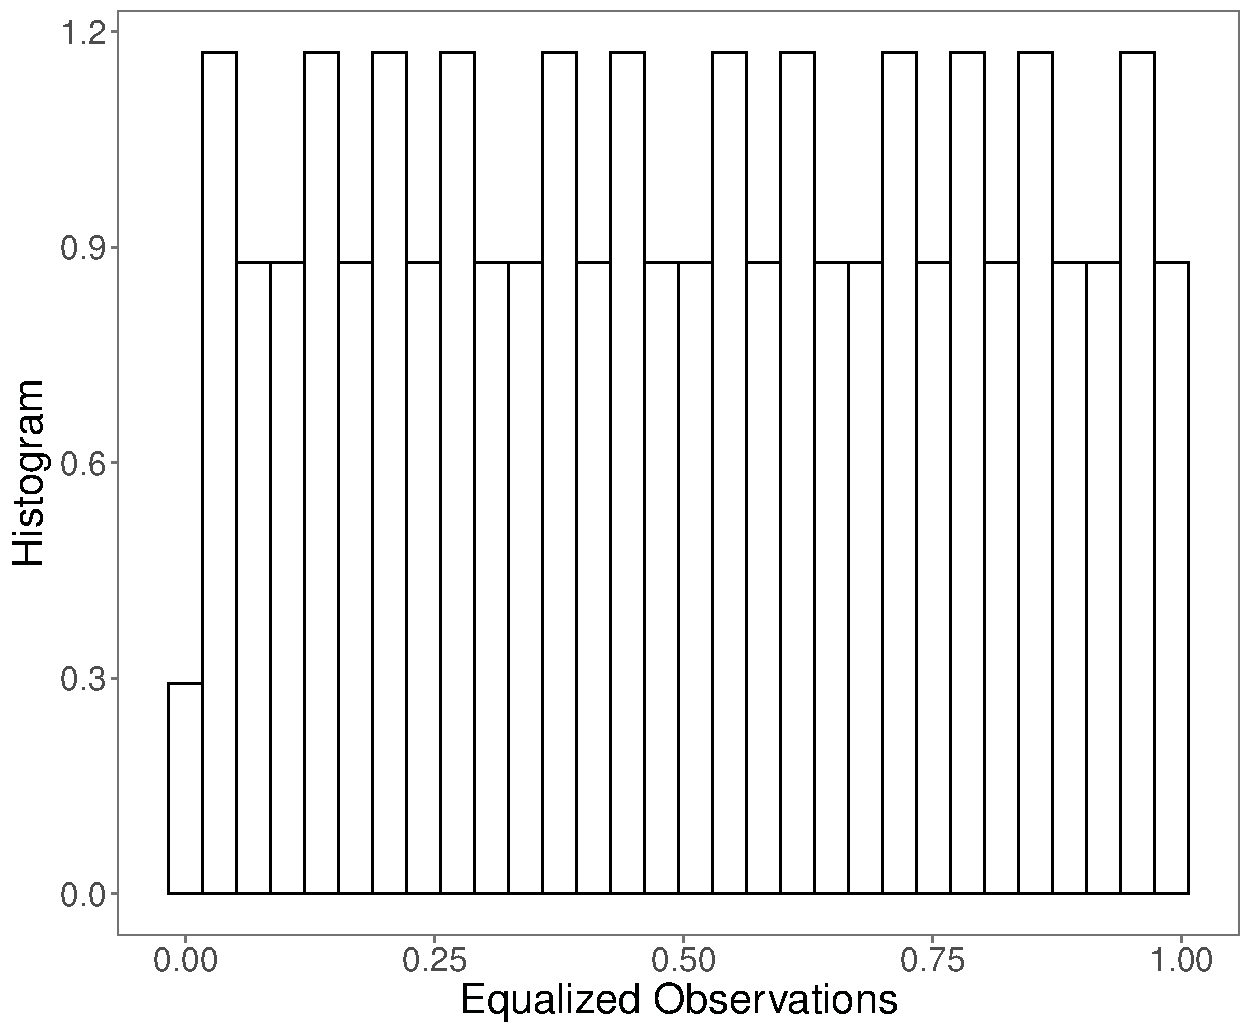
\includegraphics[width=.32\linewidth]{EqualizedHistogram}
\caption{Histogram of the original data, empirical function, and histogram of the equalized data}
\end{figure*}

The \verb|ecdf| function computes the empirical function, and returns a function that can be applied to data.
The histogram of the equalized data is fairly close to what one would expect from uniformly distributed data.
Deviations from the theoretical straight line are due to the fact that we are working with a finite sample.

But what if we do not want an image with equalized histogram?
In practice, one may find that equalized images are a bit unrealistic.
There is another theorem that nicely complements Theorem~\ref{Theo:FZ} and yields any possible distribution from a uniform law.
We will need the notion of \textit{generalized inverse functions} in order to deal equally with continuous and discrete random variables.

Assume $g\colon \mathbbm R \to \mathbbm R$ is a nondecreasing function, e.g. a cumulative distribution function.
If $g$ is continuous and strictly increasing it has an inverse $g^{-1}$.
Otherwise, define its generalized inverse function as $g^- (y) = \inf\{ x \in \mathbbm R : g(x)\geq y\}$.
If $g$ is continuous and strictly increasing, $g^{-1}$ and $g^-$ coincide.

\begin{theorem}[Inversion Theorem]\label{Theo:Inversion}
Consider the random variable $U$ uniformly distributed in $(0,1)$, and the random variable $V$ whose distribution is characterized by the cumulative distribution function $F_V$.
The random variable defined by $Y=F^-_V(U)$ has the same distribution of $V$.
\end{theorem}

\begin{proof}
The distribution of $Y$ is characterized by its cumulative distribution function $F_Y(t) = \Pr(Y \leq t)$.
But $\Pr(Y \leq t) = \Pr(F^-_V(U) \leq t)$, and applying $F_V$ to both sides of the inequality we have
$ \Pr\big(F_V(F^-_V(U)) \leq F_V(t)\big) = \Pr(U \leq F_V(t))$.
Since $U$ is uniformly distributed on the unit interval, $\Pr(U \leq F_V(t)) = F_V(t)$, so $F_Y(t) = F_V(t)$ therefore the distributions coincide.
\end{proof}

Theorems~\ref{Theo:FZ} and~\ref{Theo:Inversion} provide a powerful tool to stipulate (approximately) the marginal distribution of data.
Schematically, if we have observations from $Z$ and we want to transform them into observations of $Y$, the procedure consists of first estimating $F_Z$ by $\widehat F_Z$, and applying it to the original data.
These data will then be approximately uniform, and applying $F_Y^-$ the new observations will have the desired histogram.

Notice that $F_Y$ does not need to be specified theoretically.
It can be also computed from data.
With this, we can match the histogram of an image to that of another image;
this operation is called ``histogram matching'', and it is useful for making two data sets visually comparable.

Another important notice is that if $F$ is a cumulative distribution function, then $F^-$ is called \textit{quantile function}.

We will use as example the bright rectangle outlined in red in Fig.~\ref{Im:Oberpfaffenhofen_RGB}.
It corresponds to an urban area and, as such, it has extreme variability in the three channels.
Figs.~\ref{Fig:LinEqSpec}\subref{Fig:Linearized} and~\ref{Fig:LinEqSpec}\subref{Fig:Equalized} show the linearized and equalized versions of the data.
There is little visible in the former, and the colors are exaggerated in the latter.

\begin{figure*}[hbt]
\centering
\subfloat[Linearized data\label{Fig:Linearized}]{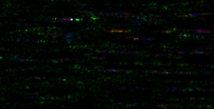
\includegraphics[width=.32\linewidth]{BrightLinearized}}\ 
\subfloat[Equalized data\label{Fig:Equalized}]{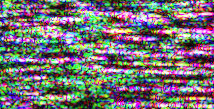
\includegraphics[width=.32\linewidth]{BrightEqualized}}\ 
\subfloat[Bands with Beta histograms\label{Fig:BetaHistograms}]{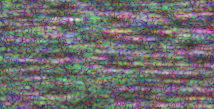
\includegraphics[width=.32\linewidth]{BetaBright}}
\caption{Examples of linearization, equalization and histogram specification of data from an urban area}\label{Fig:LinEqSpec}
\end{figure*}

The Beta distribution (see Sec.~\ref{Sec:BetaDistribution}, page~\pageref{Sec:BetaDistribution}) is a good candidate for stipulating image histograms, as it has the same support ($(0,1)$) many color models impose and is quite flexible.
Fig.~\ref{Fig:LinEqSpec}\subref{Fig:BetaHistograms} shows the result of specifying the histogram of each band as a $\mathcal B(8,8)$ distribution.
The result is more visible than the linear transformation, and less dramatic than the equalized version.

The following code illustrates how the three bands with specified Beta histograms are obtained.
Notice the use of \verb|qbeta|; this function computes the quantiles of a Beta distribution.
\begin{lstlisting}[frame=tb]
bright_rbeta <- qbeta(ecdf(bright[,,1])(bright[,,1]), shape1=8, shape2=8)
bright_gbeta <- qbeta(ecdf(bright[,,2])(bright[,,2]), shape1=8, shape2=8)
bright_bbeta <- qbeta(ecdf(bright[,,3])(bright[,,3]), shape1=8, shape2=8)
\end{lstlisting}

\section{The \texttt{imagematrix} package}

There are a few packages in \verb|R| that ease the visualization of images.
Among them, \verb|imagematrix| stands out for its simplicity.
Although it has been deprecated, and is no longer supported, we provide it with a few additional features.

The very basic rules for using \verb|imagematrix| are:
\begin{itemize}
\item image data should be in the form of a matrix of $m$ lines and $n$ columns, with either $1$ or $3$ slices; the former will be rendered as a gray-levels image, the latter as a color image;
\item the data must be in the $[0,1]$ range, otherwise it will be clipped.
\end{itemize}

Let us see an example.
\lstset{numbers=left, numberstyle=\tiny, numberblanklines=false, numbersep=5pt}
\begin{lstlisting}[firstnumber=auto,frame=tb]
source("imagematrix")
require(plot3D)

x <- 1:500
y <- 1:100
xy <- mesh(x, y)
ramp <- (xy$x + xy$y) / 600
plot(imagematrix(ramp))
imagematrixPNG(imagematrix(ramp), "../Figures/ramp.png")
\end{lstlisting}

The first line loads your local version of \verb|imagematrix|, while the second makes the \verb|plot3D| package available.
We will only use one function, namely \verb|mesh|, from the latter.
Then we build the \verb|x| and \verb|y| coordinates, and with \verb|mesh| we create their Euclidean product.
The variable \verb|ramp| stores the values of the function $(x+y)/600$, which is already bounded to $[0,1]$.
We then set the properties of an \verb|imagematrix| object to these values, and plot them.
Finally, the function \verb|imagematrixPNG| produces a PNG file tailored to the size of its input image.

\begin{marginfigure}
\centering

\includegraphics[width=.3\linewidth]{ramp}
\caption{Visualization of a ramp}\label{Fig:Ramp}
\end{marginfigure}

Fig.~\ref{Fig:Ramp} shows this ramp.
We notice that $x\in\{1,\dots,500\}$ denotes the lines, displayed from top to bottom,
while the lines are stored in $y\in\{1,\dots,100\}$ and displayed from left to right.

Some other convenient functions available in \verb|imagematrix| are:
\begin{itemize}
\item \verb|clipping|: maps any real value $z$ into $[0,1]$ by $\max\{0,\min\{z, 1\}\}$;
\item \verb|normalize|: maps all the values in the matrix $\bm z$ into $[0,1]$ by $(z - \min(\bm z))/(\max(\bm z) - \min(\bm z))$;
\item \verb|rgb2grey|: converts a color image into a gray levels one;
\item \verb|imagematrixEPS|: produces an EPS file tailored to the size of its input image;
\item \verb|equalize|: equalizes all the values;
\item \verb|equalize_indep|: equalizes the values independenty by band.
\end{itemize}
The reader is invited to browse through this code.

The book by \citet{IntroImageProcessingR} is an introduction to image processing with \texttt{R}.